\section{Быстро-медленные системы}
%%%%%%%%%%%%%%%%%%%%%%%%%%%%%%%%%%%%%%%%%%%%%%%%%%%%%%%%%%%%%%%%%%%
\subsection{Основные понятия теории быстро-медленных систем}

Во многих областях науки возникают системы, процессы в которых имеют различные временные масштабы. Если эти масштабы сильно отличаются, то переменные, отвечающие им, можно разделить на так называемые "быстрые"\, и "медленные"\,. Для описания таких процессов часто используют системы уравнений вида:
\begin{equation}
\begin{cases}
    \frac{dx}{dt} = f(x,y,\varepsilon) ,\\
    \frac{dy}{dt} = \varepsilon g(x,y,\varepsilon),
\end{cases}
\label{full1}
\end{equation}

$$(x,y) \in \mathbb{R}^n \times \mathbb{R}^m,$$
$$f,g \in C^r, r>0,$$
с малым параметром $\varepsilon$. Переменные $y$ называют медленными переменными, переменные $x$, соответственно, называют быстрыми переменными. Малый параметр 
$\varepsilon$ определяет отношение характерных временных масштабов описываемых процессов. Системы вида (\ref{full1}) называются быстро-медленными системами.
Заметим, что вводя новое "медленное"\, время $\tau = \varepsilon t$ система (\ref{full1}) принимает вид:
\begin{equation}
\begin{cases}
    \varepsilon \frac{dx}{d \tau} = f(x,y,\varepsilon), \\
    \frac{dy}{d \tau} = g(x,y,\varepsilon).
\end{cases}
\label{full2}
\end{equation}

При $\varepsilon>0$ обе системы эквивалентны, однако, при $\varepsilon = 0$ получаем так называемые "быструю"\,
\begin{equation}
\begin{cases}
    \frac{dx}{dt} = f(x,y,0), \\
    \frac{dy}{dt} = 0,
\end{cases}
\label{fast}
\end{equation}
и "медленную"\,
\begin{equation}
\begin{cases}
    0 = f(x,y,0), \\
    \frac{dy}{d \tau} = g(x,y,0),
\end{cases}
\label{slow}
\end{equation}
системы, которые не являются эквивалентными.

Очевидно, что динамика медленных переменных в быстрой системе тривиальна, и они являются параметрами для системы уравнений $\frac{dx}{dt} = f(x,y,0)$. При малых $\varepsilon$ система (\ref{fast}) хорошо описывает динамику полной системы с точностью до $O(\varepsilon)$, но только на временах порядка $O(1)$.

С другой стороны, система (\ref{slow}) хорошо описывает поведение полной системы (\ref{full2}) только на множестве нулей функции $f(x,y,0)$, называемом медленным многообразием:
$$M_0 = \{ (x,y): f(x,y,0) = 0 \}.$$

Выразив быстрые переменные на многообразии $M_{0}$ через медленные
$$x = \gamma(y),$$
и подставив в (\ref{slow}), медленная система принимает вид:
$$\frac{dy}{d \tau} = g(\gamma(y), y, 0).$$
%%%%%%%%%%%%%%%%%%%%%%%%%%%%%%%%%%%%%%%%%%%%%%%%%%%%%%%%%%%%%%%%%%%
\subsection{Представление плоской эллиптической ограниченной задачи трех тел в окрестности резонанса 3:1 в виде быстро-медленной системы}

Следует отметить, что уравнения резонансной системы (\ref{Ham_res}) могут быть приведены к виду быстро-медленной системы. Для этого рассмотрим гамильтониан вида:
$$H = \alpha \frac{\Lambda^2}{2} + \mu u \cos \lambda + \mu v \sin \lambda + \mu e_J G x + \mu F(x^2+y^2),$$

$$u(x,y) = C(x^2-y^2)+e_J Dx +e_J^2E =\frac{C}{4}(2x+\tilde \alpha)^2-Cy^2+K,$$
$$v(x,y) = 2Cxy+e_JDy =Cy(2x+\tilde \alpha),$$
$$\tilde \alpha = \frac{e_JD}{C},$$
$$K = e_J^2 E-\frac{C \tilde \alpha^2}{4},$$
которому соответствуют канонические уравнения:
\begin{equation*}
    \begin{cases}
        \frac{d \Lambda}{dt} = \mu \big( u(x,y) \sin \lambda - v(x,y) \cos \lambda \big), \\
        \frac{d \lambda}{dt} = \alpha \Lambda, \\
        \frac{dx}{dt} = -\mu \big( 2Fy+\frac{\partial u}{\partial y} \cos \lambda + \frac{\partial v}{\partial y} \sin \lambda \big), \\
        \frac{dy}{dt} = \mu \big( 2Fx+e_JG +\frac{\partial u}{\partial x} \cos \lambda + \frac{\partial v}{\partial x} \sin \lambda \big).
    \end{cases}.
\end{equation*}

Сделав несимплектическую замену $\Lambda = \sqrt \mu \Lambda_{new}$, $t_{new} = \sqrt \mu t$, получаем:

\begin{equation*}
    \begin{cases}
        \frac{d \Lambda_{new}}{dt_{new}} = u \sin \lambda - v \cos \lambda, \\
        \frac{d \lambda}{dt_{new}} = \alpha \Lambda_{new}, \\
        \frac{dx}{dt_{new}} = -\sqrt \mu \big( 2Fy+\frac{\partial u}{\partial y} \cos \lambda + \frac{\partial v}{\partial y} \sin \lambda \big), \\
        \frac{dy}{dt_{new}} = \sqrt \mu \big( 2Fx+e_JG +\frac{\partial u}{\partial x} \cos \lambda + \frac{\partial v}{\partial x} \sin \lambda \big).
    \end{cases}
\end{equation*}

В дальнейшем для удобства мы будем опускать индекс $new$. Введем новый малый параметр $\varepsilon = \sqrt \mu$. Тогда уравнения принимают итоговый вид (точка обозначает производную по $t$):

\begin{equation}
    \begin{cases}
        \dot \Lambda = u \sin \lambda - v \cos \lambda, \\
        \dot \lambda = \alpha \Lambda, \\
        \dot x = -\varepsilon \big( 2Fy+\frac{\partial u}{\partial y} \cos \lambda + \frac{\partial v}{\partial y} \sin \lambda \big), \\
        \dot y = \varepsilon \big( 2Fx+e_JG +\frac{\partial u}{\partial x} \cos \lambda + \frac{\partial v}{\partial x} \sin \lambda \big). \\
    \end{cases}
    \label{fullt}
\end{equation}

Согласно данному выше определению будем называть пару переменных $\lambda$ и $\Lambda$ быстрыми переменными, а $x$ и $y$ медленными переменными.
%%%%%%%%%%%%%%%%%%%%%%%%%%%%%%%%%%%%%%%%%%%%%%%%%%%%%%%%%%%%%%%%%%%
%\subsection{построение быстрой системы и ее описание, построение медленного многообразия его описание и картинки, построение медленной системы, ее орбит нахождение положений равновесия определенного типа}

\subsubsection{Медленное многообразие}

Медленное многообразие для системы (\ref{fullt}) представляет собой множество:
$$M_0 = \{(x, y, \lambda, \Lambda): \Lambda = 0, u(x,y) \sin \lambda = v(x,y) \cos \lambda \}.$$

Заметим, что выражение $\lambda = \arctan \big( \frac{v}{u} \big) + \pi k$ удовлетворяет условию $u \sin \lambda = v \cos \lambda$ для произвольных целых $k$. Однако, данное семейство функций терпит разрыв при переходе $u$ через 0. Данную проблему можно решить, гладко сшивая эти функции при различных $k$. Принимая во внимание то, что $\lambda\in S^{1}$, получим при этом пару непрерывных функций 
\newline $\lambda_{\pm}:\mathbb{R} \setminus \{ (x,y): u(x,y) = v(x,y) = 0 \}\to S^{1}$, значения которых отличаются на $\pi$:
$$\lambda_{+}(x,y) \equiv \begin{cases} 
        \arctan \frac{v}{u},        &  u>0, v > 0, \\
        \arctan \frac{v}{u} + \pi,  &  u<0, \\
        \arctan \frac{v}{u} + 2\pi, &  u>0, v<0,
       \end{cases}
$$
$$\lambda_{-}(x,y) \equiv \begin{cases} 
        \arctan \frac{v}{u} + \pi,  &  u>0, v > 0, \\
        \arctan \frac{v}{u} + 2\pi, &  u<0, \\
        \arctan \frac{v}{u} + 3\pi, &  u>0, v<0.
       \end{cases}
$$
Таким образом, вне точек $(x,y): u(x,y) = v(x,y) = 0$ медленное многообразие представляет собой двулистную поверхность.

Отдельный вопрос составляет случай когда $u$ и $v$ одновременно обращаются в ноль. При этом условие $u \sin \lambda = v \cos \lambda$ выполняется при произвольных 
$\lambda$ и решением является пара окружностей:
$$y_b=0,\quad x_b^{\pm}=\frac{-e_JD \pm e_J \sqrt{D^2-4EC}}{2C},\quad \Lambda = 0,\quad \lambda\in S^{1}.$$

Опишем геометрию медленного многообразия вблизи этих окружностей. Для этого разложим функции $u$ и $v$ в ряд в окрестности точки $(x_{b}^{\pm}, y_{b})$:
\begin{align*}
&u = \frac{C}{4}(2x+\tilde \alpha)^2-Cy^2+K = C(x-x_b^\pm)(2x_b^\pm + \tilde \alpha) + C(x-x_b^\pm)^2 - Cy^2,\\
&v = Cy(2x+ \tilde \alpha) = Cy(2x_b^\pm + \tilde \alpha) + 2Cy(x-x_b^\pm).
\end{align*}

Тогда в главном приближении уравнение на медленное многообразие примет вид:
$$(x-x_b^\pm)\sin \lambda = y \cos \lambda.$$
Следовательно, вблизи обеих перемычек медленное многообразие локально ведет себя как винтовая поверхность $\tg\lambda = \frac{y}{x-x_{b}^{\pm}}$.
Заметим, что при полном обходе перемычки в положительном направлении $\lambda$ увеличивается на $2\pi$

\begin{figure}[H]
\centering
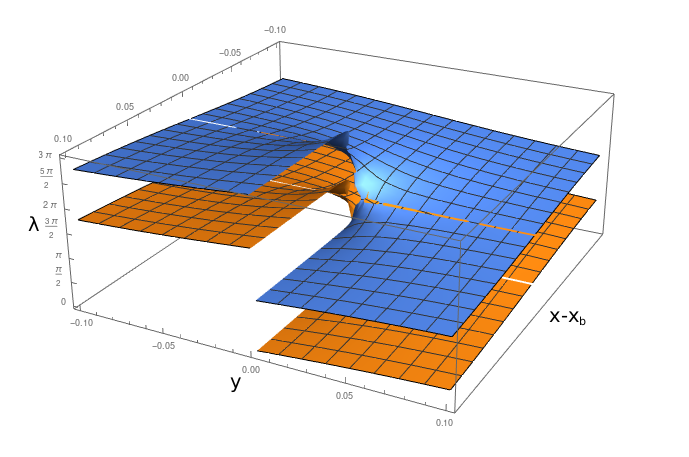
\includegraphics[scale=0.55]{img/local2.png}
\caption{Локальная струкура медленного многообразия вблизи каждой из перемычек. Разным цветом обозначены различные листы. Разрывы на каждом из листов обусловлены дефектами графопостроителя}
\end{figure}

Таким образом, мы приходим к следующему

\begin{utv}

Медленное многообразие $M_0$ плоской эллиптической ограниченной задачи трех тел в окрестности резонанса 3:1 состоит из 2 "листов"\, $M_{0,+}, M_{0,-}$, соединенных 2 "перемычками"\, $M_{0,b}^{\pm}$:
$$M_0 = M_{0,+} \cup M_{0,-} \cup M_{0,b}^{+} \cup M_{0,b}^{-},$$

\begin{eqnarray}
\nonumber
M_{0,+} = \Biggl\{ 
    \lambda = \lambda_{+}(x,y),
       \Lambda = 0,
       (x,y) \in \mathbb{R}^2 \setminus \{ (x,y): u=v=0 \}
       \Biggr\},\\
M_{0,-} = \Biggl\{ 
    \lambda = \lambda_{-}(x,y) + \pi,
       \Lambda = 0,
       (x,y) \in \mathbb{R}^2 \setminus \{ (x,y): u=v=0 \}
       \Biggr\},\\
M_{0,b}^{\pm} = \Bigl\{ y=0, x=\frac{-e_JD \pm e_J \sqrt{D^2-4EC}}{2C}, \Lambda = 0, \lambda \in S^1 \Bigr\}.
\end{eqnarray}
При этом листы $M_{0,+}, M_{0,-}$ гомеоморфны двумерной плоскости с двумя выколотыми точками, а перемычки $M_{0,b}^{\pm}$ гомеоморфны окружностям. 
\end{utv}

\begin{figure}[H]
\centering
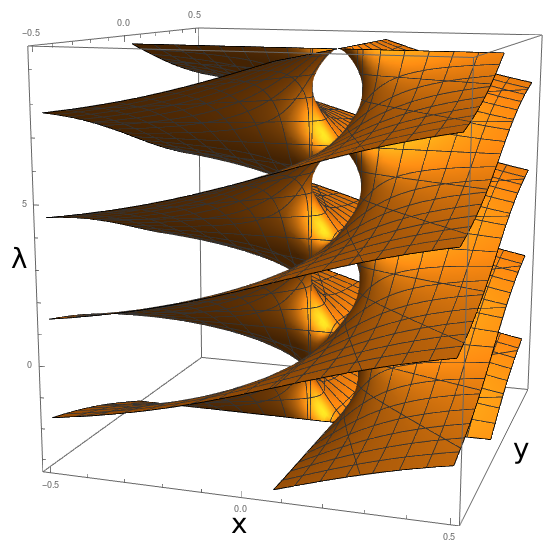
\includegraphics[scale=0.45]{img/MM.png}
\caption{Медленное многообразие}
\end{figure}

\begin{figure}[H]
\centering
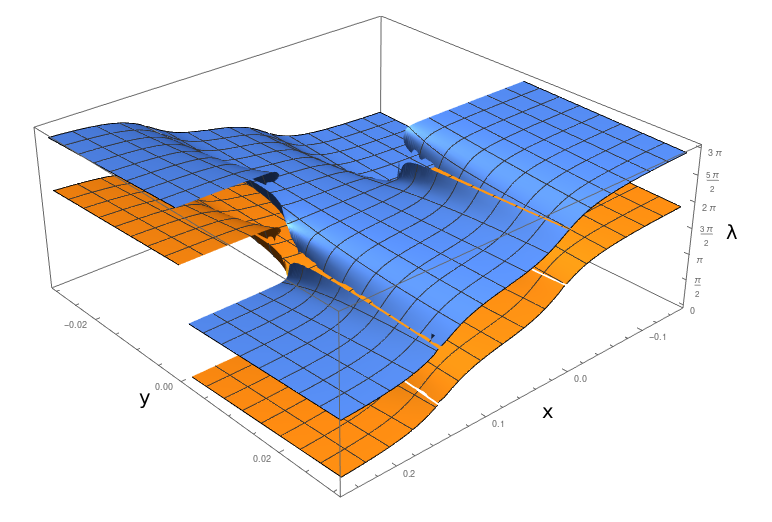
\includegraphics[scale=0.45]{img/MM2.png}
\caption{Медленное многообразие. Различным цветом обозначены различные его листы. Разрывы на каждом из листов связаны с недостатками графопостроителя}
\end{figure}


%%%%%%%%%%%%%%%%%%%%%%%%%%%%%%%%%%%%%%%%%%%%%%%%%%%%%%%%%%%%%%%%%%%
\subsubsection{Динамика быстрой системы}
Устремив в (\ref{fullt}) $\varepsilon$ к нулю, получаем так называемую "быструю"\, систему (точка обозначает производную по $t$):

\begin{equation}
    \begin{cases}
        \dot \Lambda = u(x,y) \sin \lambda - v(x,y) \cos \lambda, \\
        \dot \lambda = \alpha \Lambda, \\
        \dot x = 0, \\
        \dot y = 0.
    \end{cases}
    \label{fastreal}
\end{equation}

В силу тривиальной динамики переменных $(x, y)$ зависимость от медленных переменных функций $u, v$ будем опускать. Продифференцировав $\lambda$ второй раз по $t$ и подставляя выражение для $\dot \Lambda$, получаем уравнение:
$$\ddot \lambda - \alpha u \sin \lambda + \alpha v \cos \lambda = 0,$$
которое приводится (учитывая $\alpha < 0$) к стандартному уравнению маятника:
$$\ddot \lambda - \alpha \sqrt{u^2+v^2} \left( \frac{u}{\sqrt{u^2+v^2}}\sin \lambda - \frac{v}{\sqrt{u^2+v^2}}\cos \lambda \right) = \ddot \lambda - \alpha \beta \sin \big( \lambda - \lambda_{+}(x,y) \big) = 0,$$
где функция $\beta$ задается выражением:
$$\beta(x,y) = \sqrt{u^2+v^2} > 0.$$

Отметим, что по определению медленное многообразие является множеством неподвижных точек (положений равновесия) "быстрой"\, системы, а именно 
$(\lambda, \Lambda)  = (\lambda_{\pm}(x,y), 0)$. Для определения типа этих положений равновесия разложим правую часть уравнений (\ref{fastreal}) по формуле Тейлора в окрестности положений равновесия:
$$\begin{pmatrix}
  u \sin \lambda - v \cos \lambda \\
  \alpha \Lambda
 \end{pmatrix}
 =
 \begin{pmatrix}
  0 & \alpha \\
  \pm \beta(x,y) & 0
 \end{pmatrix}
 \begin{pmatrix}
  \lambda - \lambda_{\pm}\\
  \Lambda
 \end{pmatrix} + O((\lambda - \lambda_{\pm})^2, \Lambda^2).
$$

Из физических соображений константа $\alpha$ является отрицательной \cite{wis1}:
$$\alpha < 0.$$

Тогда собственные числа линеаризованной системы имеют вид:
\newline
для листа $M_{0,+}$:
$$\zeta = \pm i \sqrt{|\alpha| \beta},$$
\newline
для листа $M_{0,-}$:
$$\zeta = \pm \sqrt{|\alpha| \beta}.$$
В первом случае собственные значения чисто мнимые, а во втором - вещественные. Таким образом, мы приходим  следующему

\begin{utv}
Лист $M_{0,+}$ состоит из устойчивых положений равновесия быстрой системы,  а лист $M_{0,-}$  - из неустойчивых положений равновесия.

Неустойчивое положение равновесия обладает двумерной сепаратрисой, заполненной решениями вида:
\begin{align*}
&\lambda(t, t_0) = \pm 2 \arctan \sinh \big( \alpha \beta (t-t_0) \big) + \lambda_{-}(x,y),\\
&\Lambda(t, t_0) = \frac{\pm 2 \beta}{\cosh \big( \alpha \beta (t-t_0) \big)},
\end{align*}
здесь $t_{0}\in \mathbb{R}$, а выбор знака определяет направление движения по сепаратрисе.
\end{utv}

%%%%%%%%%%%%%%%%%%%%%%%%%%%%%%%%%%%%%%%%%%%%%%%%%%%%%%%%%%%%%%%%%%%
\subsubsection{Динамика медленной системы на медленном многообразии}
Заменив время на медленное $\tau = \varepsilon t$ в уравнениях (\ref{fullt}), получим (штрихом обозначается производная по $\tau$):
\begin{equation}
    \begin{cases}
        \varepsilon \Lambda' = u \sin \lambda - v \cos \lambda, \\
        \varepsilon \lambda' = \alpha \Lambda,\\
        x' = - \big( 2Fy+\frac{\partial u}{\partial y} \cos \lambda + \frac{\partial v}{\partial y} \sin \lambda \big), \\
        y' = 2Fx+e_JG +\frac{\partial u}{\partial x} \cos \lambda + \frac{\partial v}{\partial x} \sin \lambda.
    \end{cases}
    \label{fulltau}
\end{equation}

Устремив $\varepsilon$ к нулю, получаем "медленную"\, систему:
\begin{equation}
    \begin{cases}
        0 = u \sin \lambda - v \cos \lambda, \\
        0 = \alpha \Lambda, \\
        x' = -\big( 2Fy+\frac{\partial u}{\partial y} \cos \lambda + \frac{\partial v}{\partial y} \sin \lambda \big), \\
        y' = 2Fx+e_JG +\frac{\partial u}{\partial x} \cos \lambda + \frac{\partial v}{\partial x} \sin \lambda.
    \end{cases}
    \label{slowreal}
\end{equation}

В силу определения функций $\lambda_{\pm}$ выражения для $\sin \lambda$ и $\cos \lambda$ на листах медленного многообразия имеют вид:
$$\sin \lambda = \frac{\pm v}{\sqrt{u^2+v^2}},$$
$$\cos \lambda = \frac{\pm u}{\sqrt{u^2+v^2}},$$
здесь знак $+$ соответствует $M_{0,+}$, а знак $-$ соответствует $M_{0,-}$.
Подставляя их в (\ref{slowreal}), получим:
\begin{equation}
    \begin{cases}
        x' = - \big( 2Fy \pm \frac{\partial \beta}{\partial y} \big), \\
        y' = 2Fx+e_JG \pm \frac{\partial \beta}{\partial x}.
    \end{cases}
    \label{slow_sys}
\end{equation}

Данная система является гамильтоновой с гамильтнонианом:
$$H_S = F(x^2+y^2) + e_JGx \pm \beta(x,y),$$
и имеет одну степень свободы, что приводит к ее интегрируемости.

Рассмотрим множество ее неподвижных точек. Можно показать, что на каждом из листов медленного многообразия существует единственное положение равновесия:
$$
y_0^{\pm} = 0,\quad
x_0^{\pm} = \frac{e_J (\pm D - G)}{2(F \mp C)}.
$$

Линеаризуя правую часть уравнений в окрестности этой точки, получаем:
$$\begin{pmatrix}
  \frac{dx}{d \tau} \\
  \frac{dy}{d \tau}
 \end{pmatrix}
 =
 \begin{pmatrix}
  0 & -\left( 2F \pm 2C \pm \frac{2Cx_0^{\pm}+e_JD}{|u(x_0^{\pm},0)|} \right) \\
  2F \mp 2C & 0
 \end{pmatrix}
 \begin{pmatrix}
  x - x_0^{\pm}\\
  y
 \end{pmatrix} + O \big( (x-x_0^{\pm})^2, y^2 \big).
 $$
Собственные значения матрицы линеаризации имеют вид:
$$\zeta = \pm \sqrt{- \left( 2F \pm 2C \pm \frac{2Cx_0^{\pm}+e_JD}{|u(x_0^{\pm},0)|} \right)\big( 2F \mp 2C \big)} \in \mathbb{R},$$
причем, учитывая значения констант, они являются чисто вещественными, что позволяет сказать о неустойчивости данного положения равновесия на обоих листах.

Как и в случае маятника, эти неустойчивые положения равновесия обладают двумерными сепаратрисами, заполненными сепаратрисными решениями, асимптотически приближающимися к положениям равновесия при $\tau\to \pm\infty$. Для их нахождения рассмотрим линию критического уровня гамильтониана $H_S(x,y) = H_S(x_0^{\pm},y_0^{\pm})$, соответствующего неподвижной точке:
$$H_S(x_0^{\pm},y_0^{\pm}) = F(x^2+y^2)+e_JGx \pm \beta(x,y).$$

\begin{figure}[H]
\centering
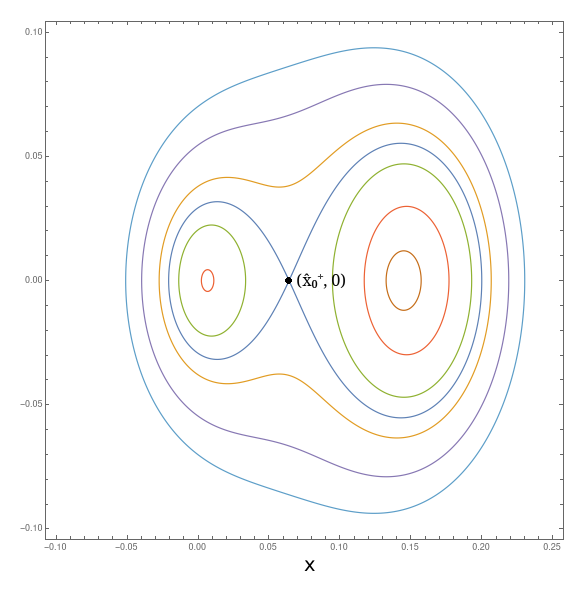
\includegraphics[scale=0.4]{img/Hlines.png}
\caption{Линии уровня гамильтониана $H_S$ на $M_{0,+}$. На $M_{0,-}$ линии уровня имеют аналогичный вид}
\label{levels_slow}
\end{figure}

Сделав замену $x = x_0^{\pm} + h$ и упростив выражение, получаем:
\begin{multline}
(F^2-C^2)(h^2+y^2)^2+2(h^2+y^2) \big(u(x_0^{\pm}, y_0)+h(2Cx_0^{\pm}+e_JD) \big) (\pm F - C)+\\ 
+ y^2 \big(4u(x_0^{\pm},y_0^{\pm})C-(2Cx_0^{\pm}+e_JD)^2 \big) = 0.
\label{eight}
\end{multline}
Сделаем инверсию относительно единичной окружности: $X=\frac{h}{h^2+y^2}$, $Y=\frac{y}{h^2+y^2}$. Тогда уравнение (\ref{eight}) принимает вид:
$$(F^2-C^2)+AX^2+2BX+(A+\delta)Y^2=0,$$
где
$$A = 2 u(x_0^{\pm}, y_0^{\pm})(\pm F - C),$$
$$B = (2Cx_0^{\pm}+e_J D)(\pm F - C),$$
$$\delta = -(2Cx_0^{\pm}+e_J D)^2.$$
Если ввести новые переменные:
$$\xi  = \left( X+\frac{B}{A} \right) \sqrt{\frac{A}{F^2-C^2-\frac{B^2}{A}}} \equiv \omega \left( X+\frac{B}{A} \right),$$
$$\eta = Y \sqrt{\frac{-(A+\delta)}{F^2-C^2-\frac{B^2}{A}}} \equiv \sigma Y,$$
то уравнение критического уровня может быть переписано следующим образом:
\begin{equation}
\label{hyper}
\xi^2-\eta^2=1.
\end{equation}
Таким образом, в переменных $(\xi, \eta)$ линия уровня гамильтониана $H_S(x,y) = H_S(x_0^{\pm},y_0^{\pm})$ есть гипербола. В первоначальных переменных  $(x, y)$, т.е. до инверсии относительно единичной окружности, данная кривая имеет форму "восьмерки"\, (см. рис. \ref{levels_slow}).

Введем следующую параметризацию полученной кривой с помощью переменной $f$:
$$\xi = \ch f,$$
$$\eta = \sh f,$$
$$\xi^2-\eta^2 = \ch^2f - \sh^2f = 1.$$
Теперь для нахождения сепаратрисного решения необходимо определить зависимость $f$ от времени $\tau$. Для этого рассмотрим:
\begin{equation}
\label{der_x_1}
x' = \frac{\partial x}{\partial X}X'+\frac{\partial x}{\partial Y}Y' = \frac{Y^2-X^2}{(X^2+Y^2)^2}X' + \frac{-2XY}{(X^2+Y^2)^2}Y' = f' \sh f \frac{Q(\ch f)}{P^2(\ch f)},
\end{equation}
где
$$P(\ch f) \equiv X^2+Y^2 = \ch^2 f \left( \frac{1}{\omega^2} + \frac{1}{\sigma^2} \right) + \frac{-2B }{\omega A}\ch f + \left( \frac{B^2}{A^2}-\frac{1}{\sigma^2} \right),$$

$$Q(\ch f) \equiv  -\frac{\ch^2 f}{\omega} \left( \frac{1}{\omega^2}+\frac{1}{\sigma^2} \right) + \frac{2B}{A} \ch f \left( \frac{1}{\sigma^2}+\frac{1}{\omega^2} \right) - \frac{1}{\omega} \left( \frac{1}{\sigma^2} + \frac{B^2}{A^2} \right).$$

С другой стороны, подставляя (\ref{eight}) в первое уравнение системы (\ref{slow_sys}), получаем:

$$x' = -\left( 2Fy \pm \frac{\partial \beta}{\partial y} \right) = -2Fy \mp \frac{1}{\beta} \left( u \frac{\partial u}{\partial y} + v \frac{\partial v}{\partial y} \right) = $$

$$ = \frac{y \Big(2(C^2-F^2)(x^2+y^2) + 2x(2Cx_0+e_J D)(C \mp F) + (2Cx_0+e_J D)^2 + 2u(x_0, y_0)(-C \mp F)  \Big)}{F(x^2+y^2) \pm u(x_0, y_0) \pm x(2Cx_0+e_J D)}.$$

Тогда в терминах переменной $f$ получаем
\begin{equation}
\label{der_x_2}
x' = \frac{\sh f}{\sigma P(\ch f)} \frac{R(\ch f)}{S(\ch f)},
\end{equation}
где
$$R(\ch f) \equiv P(\ch f) \left( 2 u(x_0,y_0)(-C \mp F)+(2Cx_0+e_J D)^2 \right) +$$ 
$$ + 2 \left( \frac{\ch f}{\omega} - \frac{B}{A} \right)(2Cx_0 + e_J D)(C \mp F) + 2(C^2-F^2),$$
$$S(\ch f) \equiv \pm u(x_0,y_0) P(\ch f) \pm \left( \frac{\ch f}{\omega} - \frac{B}{A}\right) (2Cx_0+e_J D) + F.$$
Сравнивая выражения (\ref{der_x_1}) и (\ref{der_x_2}), получаем дифференциальное уравнение на $f$:
\begin{equation}
\label{der_f}
f' = \frac{1}{\sigma} \frac{R(\ch f) P(\ch f)}{S(\ch f)Q(\ch f)}.
\end{equation}
Заметим, что $P, Q, R, S$ являются полиномами второго порядка переменной $\ch f$.
Интегрируя уравнение (\ref{der_f}), имеем:
\begin{equation*}
\tau -\tau_0 = \sigma \int_{f_0}^f \frac{S(\ch f) Q(\ch f)}{R(\ch f)P(\ch f)} df = 
\end{equation*}
\begin{equation} = (f-f_0)\frac{\mp 2u(x_0^{\pm}, y_0^{\pm}) \frac{\sigma}{\omega}}{2u(x_0^{\pm},y_0^{\pm})(-C \mp F)+(2Cx_0^{\pm} + e_J D)^2} + \sigma \int_{f_0}^f \frac{L(\ch f)}{R(\ch f) P(\ch f)} df,
\label{f_tau}
\end{equation}
где $L$ некоторый полином 3 степени.

\begin{utv}
На обоих листах $M_{0,k}, k=+,-$ медленная система (\ref{slow_sys}) имеет неустойчивое положение равновесия $(x,y) = (x_0^{\pm},y_0^{\pm})$. Это положение равновесия порождает двумерную сепаратрису, заполненную решениями вида:
$$x(\tau,\tau_{0}) = x_0 + \frac{\frac{\ch \big( f(\tau-\tau_{0}) \big)}{\omega} - \frac{B}{A}}{P \Big(\ch \big( f (\tau-\tau_{0}) \big) \Big)},$$
$$y(\tau, \tau_{0}) = \frac{\sh \big( f(\tau-\tau_{0}) \big)}{\sigma P\Big(\ch \big( f (\tau-\tau_{0}) \big) \Big)},$$
где $\tau_{0}\in \mathbb{R}$, а функция $f(\tau)$ задается выражением (\ref{f_tau}).
\end{utv}